\documentclass[submit,techrep,noauthor]{ipsj}

\usepackage[dvipdfmx]{graphicx}
\usepackage{latexsym}
\usepackage{url}
\usepackage{xcolor}
\usepackage{listings}
\usepackage{amsmath,amssymb}
\usepackage{tabularx}
\usepackage{stfloats}
\usepackage{booktabs}
\usepackage{threeparttable}
\usepackage{caption}

\newcounter{patternID}

% ソースコード例を載せるためのあれこれ
\definecolor{lightred}{RGB}{255,230,230}
\definecolor{lightgreen}{RGB}{230,255,230}

\lstset{
    basicstyle=\small\ttfamily,
    abovecaptionskip=0pt,
    captionpos=b,
    frame=tb,
    framexleftmargin=2em,
    numbers=left,
    numberstyle={\scriptsize},
    xleftmargin=\parindent,
    escapechar=|
}

%ListingのキャプションがFigureになってしまうのをListingに直すコマンド
\usepackage{caption}
\makeatletter
\let\MYcaption\@makecaption
\makeatother
\usepackage{caption}
\makeatletter
\let\@makecaption\MYcaption
\makeatother

\newcommand{\todo}[1]{\colorbox{yellow}{{\bf TODO}:}{\color{red} {\textbf{[#1]}}}}
\newcommand{\memo}[1]{\colorbox{magenta!30}{{\bf MEMO}:}{\color{red!50} {\textbf{[#1]}}}}
\newcommand{\ihara}[1]{\colorbox{green}{{\bf IHARA}:}{\color{blue} {\textbf{[#1]}}}}

\def\Underline{\setbox0\hbox\bgroup\let\\\endUnderline}
\def\endUnderline{\vphantom{y}\egroup\smash{\underline{\box0}}\\}
\def\|{\verb|}
%

\def\Underline{\setbox0\hbox\bgroup\let\\\endUnderline}
\def\endUnderline{\vphantom{y}\egroup\smash{\underline{\box0}}\\}
\def\|{\verb|}

\begin{document}


\title{大規模言語モデルによるソースコード生成のための反復的な要件統合と最適化プロセス}


\affiliate{WU}{和歌山大学\\
Wakayama University, 930 Sakaedani, Wakayama 640--8510, Japan}

\author{豊嶋 浩基}{Toyoshima Hiroki}{WU}[s276157@wakayama-u.ac.jp]
\author{伊原 彰紀}{Ihara Akinori}{WU}[ihara@wakayama-u.ac.jp]
\author{田井 聖凪}{Tai Sena}{WU}[s2310137@wakayama-u.ac.jp]

\begin{abstract}
大規模言語モデル (LLM) はソフトウェア開発自動化に大きく貢献するが,複雑な要件を持つソフトウェア開発の実現には課題が多い.
本研究は,このような課題の解決に向けて,自然言語からソースコードを自動生成するマルチエージェント型のプラットフォームChatDevを拡張する.具体的には,few-shot学習を用いた要件の細分化と各ステップの開発を行うLLMに要件の全体概要の学習によるソースコード自動生成並びに,生成ステップ毎の差分行数に基づく要件の統合及び,統合結果を分割例と再分割を組み合わせた反復的に進める開発プロセスを提案する.
ケーススタディとして,競技プログラミングサイトであるAtCoderの問題を題材に,この提案手法を実施した結果,few-shot学習と全体概要の共有の組み合わせによりテスト通過率が向上し,統合に基づく要件の再分割により生成されたソースコードはさらにテスト通過率が向上することを明らかにした.

% と段階的開発を実施した.これにより,入出力テストに基づいた性能の向上が確認できた一方で,局所的な最適化に留まり,システム全体の品質に課題を残す.
% そのため本研究では,分割された要件の統合と反復的改善の概念を組み合わせた新たな開発プロセスを提案する.具体的には,分割・生成されたソースコード群を対象に,全体の整合性を評価し,再統合と洗練を行うイテレーションを導入する.この反復的な最適化プロセスは,複雑なソフトウェア要件に対するソースコード生成品質を一段階引き上げるための,新たな開発指針となることを目指す.
\end{abstract}

\maketitle

%%%%%%%%%%%%%%%%%%%%%%%%%%%
%1
\section{はじめに}
%%%%%%%%%%%%%%%%%%%%%%%%%%%

大規模言語モデル (LLM) 技術の急速な発展に伴い\cite{Growing_LLM},LLMはこれまで人間が時間や労力をかけていたタスクの自動化を実現し,幅広い分野の作業を効率化する技術として関心を集めている.
ソフトウェア開発においても,コードレビュー,リファクタリング,テストケース生成など,様々な場面において飛躍的に生産性を向上することが確認されている\cite{LLM_CodeReview}\cite{LLM_Refactoring}\cite{LLM_Gene_Test}.
その中でも,開発者の意図や要件をプロンプトとして提示し,ソースコードを自動生成するタスクに対する期待が大きい\cite{LLM_CodeGeneration}.

LLMは,自然言語で記述された要求文に基づきソースコードの自動生成を実現し,昨今では複雑で,大規模なソフトウェア開発の自動化に向けた研究が進められている\cite{LLM_CodeGeneration}.
規模が小さいソフトウェアの要求は実現できる一方で,ソフトウェア要件が複数内包し,それぞれが相互に依存し合う大規模なソフトウェア要件を満たすソースコード生成には課題が多い.
従来研究ではソフトウェア要件が複雑になると,LLMが十分に推論せずに,短絡的なソースコードを生成することが示されている\cite{IllusionApple}.
例えば,仕様の一部が欠損している場合や,要件の文脈を正しく理解できない場合には,ロジック誤りが生じることがある.
これは,要件文から要求を抽出し,それらを基にソースコードを生成する,という流れをLLMが実施するが,複雑な要件からソースコードを生成する場合,LLMは追加の学習データなしに正しく要求を抽出する事が困難である.
LLMは要件を基にソースコードの生成を行うため,要件の抽出誤りが不完全なソースコードを生成する原因の1つであると考えられる.

LLMの理解や推論を補助するプロンプト技術として,思考の過程を明示的に示すChain of Thought (CoT) や,要求を満たす例を少数提示するfew-shot学習が用いられている\cite{LLM_fewshot}.これらは局所的な推論の補完や思考パターンの学習には有効である一方で,プログラミング言語のように記述方法や実装方法によって同一の要件に対して多様な解が存在する領域では,これらの手法のみでは十分な性能を発揮しにくい.

これに対して先行研究では,全体の流れから要件を抽出するフェーズと,それらを基にソースコードを生成するフェーズの2つに分割する手法が取り入れられている\cite{tosem}.
前者では,大量のデータ収集やそれに対するラベリング,再学習などを要するファインチューニングと比較して,追加学習することなくLLMの挙動を制御できるfew-shot学習が採用されている.
当該研究では,複数の各機能を並列に生成し,生成されたすべてのソースコード片の結合時に,各断片における前提が共有されず,関数やファイル単位での依存関係や,グローバル変数の扱いや,エラーハンドリングなど,ソースコード単位での整合性が破綻する課題に言及している.


本研究では,従来研究\cite{tosem}の要求抽出の不安定さや,段階的開発におけるソースコードの断片化の課題解決に向けて,複雑な要件の細分化および,細分化した要件ごとの開発における全体整合を実施することでソースコード自動生成を実現する.
さらに,細分化した要件をベースとして生成したソースコードを評価し,要件の統合と再分割によるソースコード自動生成を複数回繰り返すことでプロンプト作成の最適化を目指す開発プロセスを提案する.
本手法により,各工程においてLLMに対して全体概要を明示的に提示し,分割した要件の統合と再分割を繰り返すことで,マルチエージェント型ソースコード自動生成の品質を向上を期待する.


論文構成は以下の通りである.\ref{sec:related}章で本研究で使用するフレームワークやキーアイディアのベースとなる関連研究について,\ref{sec:method}章ではそれらに基づいたアプローチを述べ,\ref{sec:evaluation}章でそのアプローチに関する実験設定やRQを列挙し,\ref{sec:result}章でそれに対する結果を提示する.\ref{sec:discussion}章で考察と妥当性の脅威について議論した上で,\ref{sec:conclusion}章で結論を述べる.


%%%%%%%%%%%%%%%%%%%%%%%%%%%
%2
\section{関連研究}
\label{sec:related}
%%%%%%%%%%%%%%%%%%%%%%%%%%%

%2.1
\subsection{ChatDev: マルチエージェントによる段階的開発フレームワーク}
LLMを活用したソフトウェア開発の全プロセスの自動化を目的としたシステムとして,MetaGPT,AutoDevなどの開発が盛んに進められている\cite{metagpt}\cite{autodev}.
本システムは,ソフトウェア開発プロセスにおける各工程(要求定義,設計,実装,テスト,保守)を自然言語理解と生成能力により自動化する仕組みである.
本研究では,各工程の役割を担うLLMエージェントがそれぞれ要件定義から実装までを実現するChatDev\cite{qian-etal-2024-chatdev}を用いる.

ChatDevは,要件定義,設計,実装をウォーターフォールモデルに則って開発を進める過程で,各工程においてプログラマやプロダクトマネージャといった役割を与えられた2つのLLMエージェントが対話しながら開発を行うプラットフォームである.
各工程では,開発を担当するエージェントが,プロンプトで与えられた要件文,または前工程で生成された成果物(ソースコード)に基づき,新たな成果物を生成する.生成した成果物は別の検証を担当するエージェントと共有される.
共有を受けたエージェントは,成果物を検証し,開発と検証を担当するエージェント間で合意形成を図って,成果物を完成する.

ChatDevの枠組みは,各工程のタスクが明確である点や,フレームワークがオープンソースとして公開されており,自体の構造の確認や書き換えが可能であるため,拡張性に優れている.
一方で,各工程で開発を担当するLLMに対して,同一の要件(プロンプト)が与えられるため,多数の機能を内包するような複雑・大規模な要件の場合,各フェーズでのタスクの粒度が大きくなり,不完全なソースコードが生成されやすくなってしまう.


%2.2
\subsection{LLMによるソフトウェア開発自動化の課題}
Shojaeeら\cite{IllusionApple}は,複雑度の制御が可能かつ,解法が明確な数学的パズル問題を用いて,LLMの最終的な解とそこに至るまでの推論過程を調査した.
その結果,難易度が上昇するにつれて正答率は緩やかに低下すると同時に,複雑度が一定の閾値を超えるまでは推論過程での思考量が増加した.
一方で,複雑度が一定の閾値を超えると思考量は急減し,推論が打ち切られ,LLMの推論精度が低下することが確認された.
加えて,推論過程の調査により,複雑度が低い場合は正解まで早く到達するが,その後も不要に探索を続けてしまう過剰な推論ステップを踏むことが確認された.
このようなLLMの挙動は,高い推論能力を要する自然言語からのソースコード自動生成においても同様に発生し得るものである.
複数の要求を内包する複雑な要件文からは,依存関係の見落としや,断片化したソースコードの生成により,全体整合性の破綻が発生しやすい.

Jiangら\cite{tosem}は,few-shotによりLLMを用いて要求文から小さな実装単位の要件に分割する「計画フェーズ」と,分割後の要件を基に開発を行なっていく実装フェーズを組み合わせた手法を提案している.
計画フェーズにおいてfew-shot学習として分割例を入力して要求文を分割することで,分割した要件を最適な粒度に均一化する事を目指している.
このように,当該研究が提案する分割後要件の粒度の最適化を図る「要件の細分化」と「細分化後要件の統合と再分割」は,LLMの推論の最適化プロセスの1つとして重要であると考えられる.
さらに実装フェーズにおいては,分割後の要件文を個別に並行的に実装していくのではなく,開発順序を定めるガイドとして順次参照しつつ,全体を一体として一括で生成する構成が最も高性能であると報告されている.
これは,複数の要件からソースコードに並行して生成し,最終的に結合を行う方式は,コンテキストの欠如により,インタフェースやデータ構造の不整合が発生する可能性が高くなると言及されている.

本研究では,プロンプトとその時点で作成された成果物から開発を実施する構造をとるChatDevを用いる事で,段階的開発を実施しながらも,断片化を回避する手法について調査する.


%%%%%%%%%%%%%%%%%%%%%%%%%%%
%3
\section{要件分割と要件統合に基づく段階的ソースコード生成}
\label{sec:method}
%%%%%%%%%%%%%%%%%%%%%%%%%%%

%--------------------
\begin{figure*}[t]
    \centering
    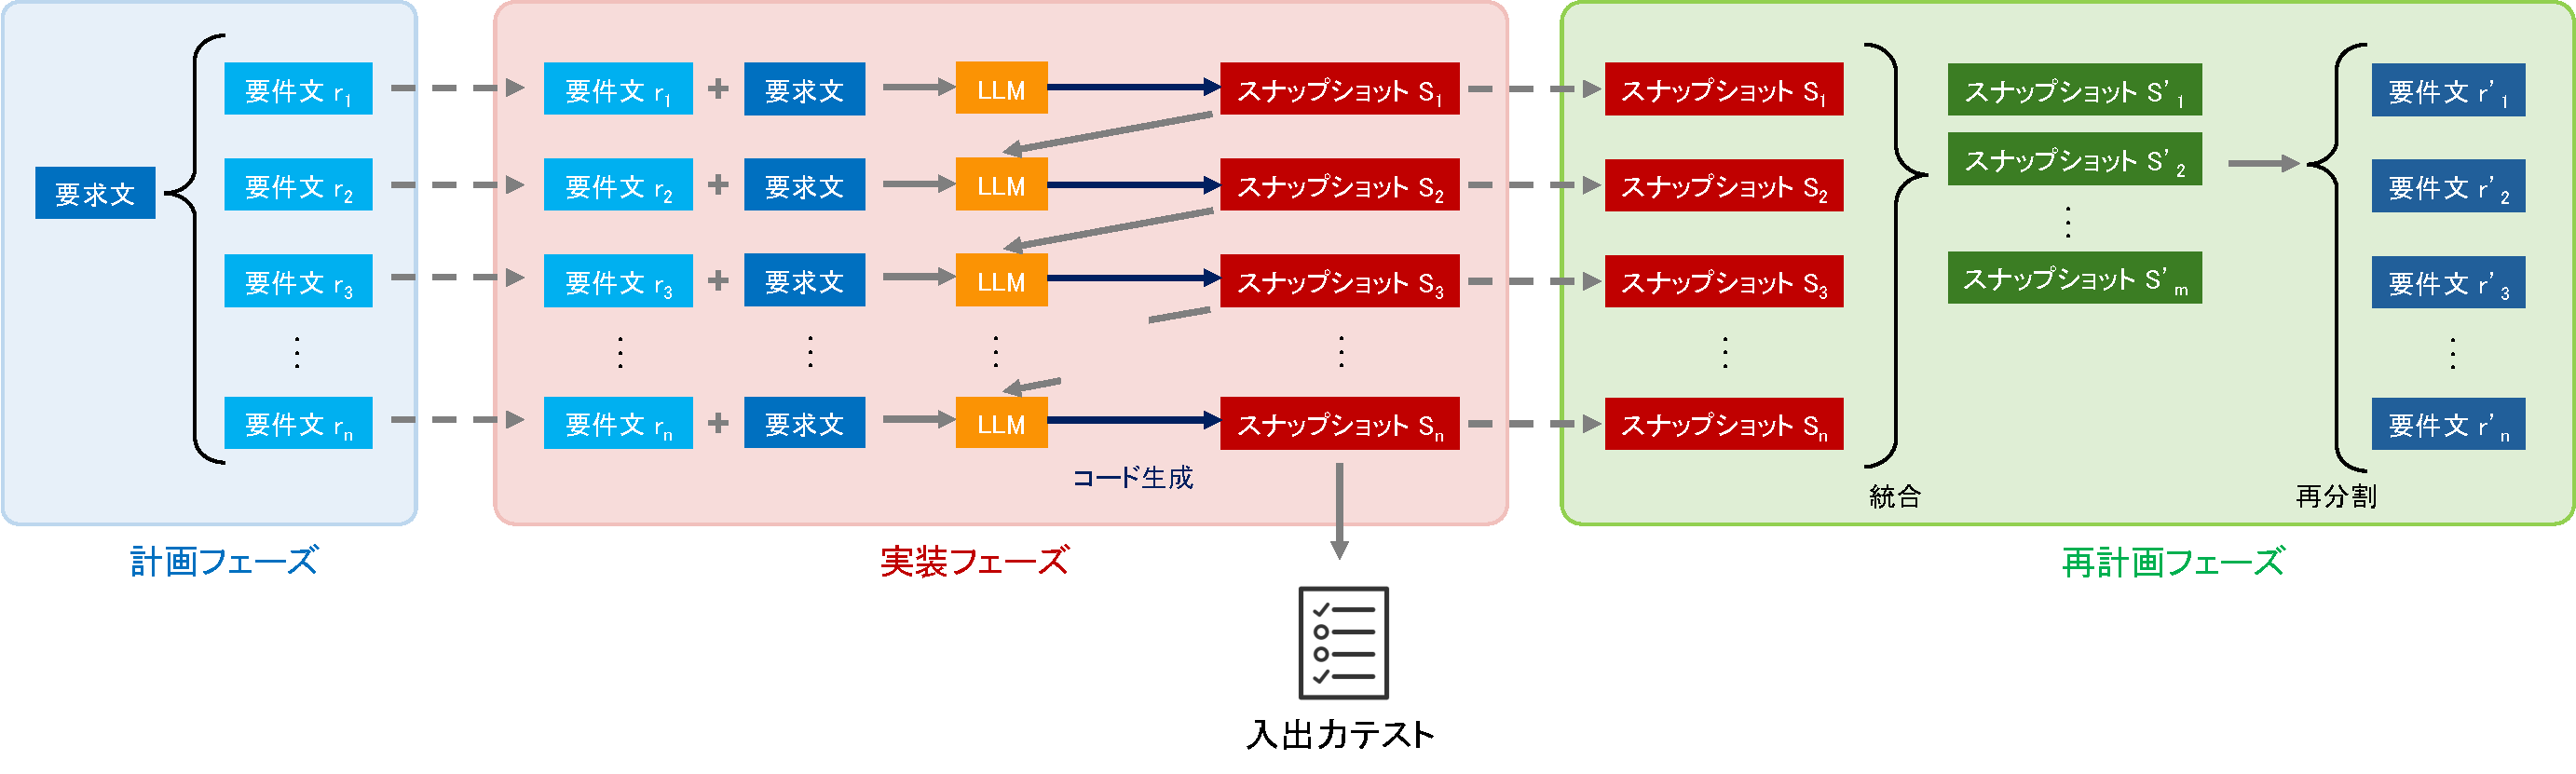
\includegraphics[width=1.0\linewidth]{./Toyoshima_fig/approach_abst_v3.pdf}
    \caption{アプローチの概略図}
    \label{approach_abst}
\end{figure*}
%--------------------

\subsection{概要}
従来のChatDev\cite{qian-etal-2024-chatdev} は,単一のプロンプトから設計,実装,コードレビュー,テストのようにウォーターフォールモデルの流れを実施し,ソースコードを生成している.ChatDevは従来研究\cite{tosem}において,要求文を分割して,段階的に開発を進める仕組みを持たない.それに対して本研究では,分割された要件文からそれに対応する開発が実施できるように構造を拡張し,ソフトウェア生成の精度向上を目指す.
具体的には,本手法は要求文を要件に細分化する「計画フェーズ」と,細分化された要件を基にソースコードの生成を行う「実装フェーズ」,実装フェーズで生成されたソースコードを基に要件の統合と再分割を実施する「再計画フェーズ」の3フェーズで構成する.図\ref{approach_abst}は,本手法の概略図を示す.

計画フェーズは,ソフトウェアの要求文をLLMに対してfew-shot学習を実施することで,要求文を要件に細分化する.

実装フェーズは,細分化された要件をウォーターフォールモデルの流れで段階的にそれぞれ実装を進める.各ステップでLLMには3種類のデータを入力する.
(1) 実装する要件文,(2) 分割前の要求文,(3) 2つ目以降の要件の実装時には,それまでに開発された成果物.
これらのデータに基づき,各要件をLLMにより実装する.

再計画フェーズでは,分割されたソースコードの結果を基に要件の統合を実施し,統合した要件をLLMに学習させる事により要求から要件への再分割を実施する.

これらにより,入出力テストの通過率向上を目指す.

% 分割済みの要件から段階的に開発を進める各ステップにおいて,LLMには開発を担当する分割後の小要件とそれまでに開発された成果物(設計・ソースコード・テストなど)に加えて,分割前の要件を全体概要が提示され,それを基に開発が進められる.ここでいう全体概要とは,細分化した要件を論理順に統合したものを指す.このような全体概要を開発を担当する全てのLLMに与える事により,2.3節で議論されていた開発の断片化を防ぎ,全体整合性の担保を目指す.

% 本論文におけるアプローチでは,2.3節の方針に基づいて,自然言語の要件文をLLMを用いて細分化を行う「計画フェーズ」と,2.1節で示したChatDevの機能を拡張し,段階的に開発を実施する「実装フェーズ」の2フェーズをベースとする.

% また,2フェーズにより生成されたソースコードに基づいて,計画フェーズで細分化した要件の統合及び,細分化を実施する.統合により分割粒度の最適化を図り,再分割により依存関係や,要求の補正を狙いとする.具体的な分割規則や,拡張設計及び統合・再分割の指標は後続の節で説明する.

% 図\ref{approach_abst}で示す〜〜.\todo{どこかに入れる}


% %3.1
% \subsection{全体概要に基づく段階的開発}
% 本研究では,分割済みの要件から段階的に開発を進める各ステップにおいて,LLMには開発を担当する分割後の小要件とそれまでに開発された成果物(設計・ソースコード・テストなど)に加えて,分割前の要件を全体概要が提示され,それを基に開発が進められる.ここでいう全体概要とは,細分化した要件を論理順に統合したものを指す.このような全体概要を開発を担当する全てのLLMに与える事により,2.3節で議論されていた開発の断片化を防ぎ,全体整合性の担保を目指す.

%3.2
\subsection{計画フェーズ}
要求文の分割は,異なる開発者が行うと分割粒度が異なることも少なくない\cite{split_size}.LLMも同様に,共通した粒度で要求文を要件に分割することは容易でない.
本手法では,評価対象とは別のソフトウェア開発における要求文を手動で要件に分割した結果をfew-shot学習を行ったLLMモデルを用いて,要求文の分割を実施する.
Listing~\ref{sample_split}は,要求文を分割するプロンプトの一部を抜粋したものである.
few-shot学習に用いるソフトウェア開発データは,分割後の要件に基づきLLMで生成したソースコードが入出力テストを全て通過しているものとする.
また,分割時に「重要な機能であればあるほど前方に配置する」という命令を与え,ソースコードの主要処理から実装するように実装する順番もLLMが決定する.
実装する順に要件には,$r_1$,$r_2$,$r_3$,\dots,$r_n$のようにラベルを付与する.

%----------------------------------
\begin{lstlisting}[caption=要求分割のためのプロンプト(一部抜粋), label=sample_split, captionpos=t, columns=fullflexible, breaklines=true]
# Role
You are an expert in software requirements elicitation.

# Objective
From an AtCoder problem statement and its constraints, extract the requirements and split them into 10 or fewer subtasks.

# Requirements
- Identify the input format and state how it will be handled in the first requirement.
- Decide which function to pass the given arguments to, and name functions/variables wherever possible.
- Mention the output format in the last requirement.
- Think of this as converting a story-like text into a list of implementable events.
- Return only the subtask list (no extra commentary).
\end{lstlisting}
%----------------------------------

% few-shotによる要件細分化の安定性を図るため,本研究では著者が要件文を手動で小要件群に分割し,その分割に基づいてLLMにソースコードを生成する.そのソースコードが用意した入出力テストを全て通過した場合に,その手動で行った分割は「正しい分割」である,と定義しする.その後に,分割前の文章と分割後の文章をペアとして,few-shotの例としてLLMへ提示する.2.3節の方針に基づき,ここで与える分割例の数は8件と固定する.その後,few-shot学習を実施したLLMに対して未分割の要件を与え,分割を実施する.この際,分割数の最大数は,分割のコストを考慮し,最大数を10個に制限する.また,分割例と共「重要な機能であればあるほど前方に配置する」という命令を与え,コア機能から開発を実施し,段階的に機能を拡張する,と言た構造とする.

%3.3
\subsection{実装フェーズ}

実装フェーズは,各要件を満たすソースコードをLLMを用いて生成する.
Jiangらは,分割した要件のみに基づき,各要件を実現するソースコードを並行して生成する場合,要求間の断片化が発生し,全体整合性が崩壊するという課題が発生している\cite{tosem}
本研究は,要件$r_1$に加え,要求文をLLMに入力し,ソースコードを生成する.
Listing~\ref{programmer_sample}は,開発を担当するLLMへ与えるプロンプトの一部を抜粋したものである.
ここで生成されたソースコード一式をスナップショット1 ($S_1$) とする.次の要件要件$r_2$は,要求文と前の要件$r_1$で生成したスナップショット1$S_1$を入力とし,ソースコードを生成する.
ここで生成されたソースコード一式をスナップショット2 ($S_2$) とする.
このように,本研究では従来研究のような要件のみでソースコードを生成するのとは異なり,要求文と前の要件で生成したスナップショットも入力として用いる.

%----------------------------------
\begin{lstlisting}[caption=実装を行うLLMへ与えるプロンプト例, label=programmer_sample, captionpos=t, columns=fullflexible, breaklines=true]
"Programmer_2": [
    "You are Programmer_1 at ChatDev. Focus subtask: {subtask2}.",
    "The overall outline of the project is as follows: {overall_task}",  
    "Strictly follow the current phase's Output rules.",
    "Constraints: single file `main.py`; STDIN/STDOUT only; stdlib only; no extra logs.",
    "Respect any required region markers (e.g., '# [SUBTASK 2 START]' / '# [SUBTASK 2 END]'); do NOT add `__main__` unless asked.",
    "Output EXACTLY ONE file in the requested format: start with 'FILENAME: main.py' then a single code block."
]
\end{lstlisting}
%----------------------------------

%3.4
\subsection{再計画フェーズ}
再計画フェーズでは,スナップショットの追加行数に基づく要件の統合と,統合した結果を用いた再分割を実施する.

2.2節で示したように,要件に対する実装量が過度に小さい場合,LLMの注意資源や推論能力を必要以上に消費し,意図しない要件を実装する可能性が存在する\cite{tosem}.
本研究では,各要件に対して生成されたソースコード規模が小さい場合,ソースコード生成後に要件の分割粒度を再検討し,要件を統合して再生成する.
本研究では,各要件の重要度をその要件$r_i$ を実装するステップで新規に追加・修正された行数を用いて評価し,その重要度を用いて要件の統合の判断基準として使用する.
具体的には,問題毎の要求から分割された要件の総数をn,$i$番目の要件$r_i$に基づき生成したソースコードのスナップショット$S_i$において,ソースコードの総行数を$LoC_i$とする.連続する2つのスナップショット対を$S_{i-1}$から$S_i$までで追加及び修正された行数を$\Delta LoC_i = LoC_i - LoC_{i-1}$ とする.

式(\ref{form:delta})で算出した差分行数$\Delta LoC_i$が,本研究で決定した閾値を下回ると,要件$r_i$は直前の要件$r_{i-1}$と統合する.

\begin{equation}\label{form:delta}
    \Delta LoC_i \leq LoC_n / n
\end{equation}

その後に,統合した要件群を基に再度ソースコードを生成し,統合の可否について調査を実施し,テストを通過したケースの統合後の要件を取得する.
取得した要件の中から無作為にサンプルを抽出し,計画フェーズと同様にfew-shot学習として分割例を入力し,要求から要件への再分割を実施し,再分割された要件からソースコードを再生成する.

% 以上のような統合と再分割により,分割粒度や要件の並び順などの最適化を目指す.

%%%%%%%%%%%%%%%%%%%%%%%%%%%
%4
\section{評価実験}
\label{sec:evaluation}
%%%%%%%%%%%%%%%%%%%%%%%%%%%

%4.1
\subsection{データセット}
本研究では,満たすべき要件が自然言語で明確に記述され,生成したソースコードを検証可能なデータセットとして,競技プログラミングサイトであるAtCoderの問題を対象に評価実験を行う.
特に,few-shot学習のために問題8問(C問題4問とD問題4問)を使用し,評価実験のために200問(C問題とD問題をそれぞれ100問)の問題を使用する.難易度の低い問題では要件の分割により,タスク粒度が過度に小さくなってしまう可能性を考慮して,C問題とD問題を対象とする.
各問題は2件から4件程度の入出力サンプルを備えており,これを評価用テストとして活用し,生成したソースコードの評価に用いる.
% 満たすべき要件が自然言語で書かれた問題文や,生成されたソースコードを評価するための入出力セットが備わっていることから競技プログラミングサイトであるAtCoder\cite{AtCoder}より541件の入出力テストをもつ200問の問題を取得した.
% 尚,難易度の低い問題では分割の必要がないことから,難易度はC問題,D問題からそれぞれ100問ずつ取得した.
また,LLMの事前学習に用いられる学習用データの多くは英語が中心であり,他言語と比較して性能の差が挙げられる\cite{LLM_En} .要件の理解の一貫性や再現性を担保するために,問題文などの自然言語は全て英語の問題を対象とする.

%4.2
\subsection{実験設定}
計画フェーズでは,著者が手動で要求文から要件分を作成し,それらをLLMにfew-shot学習させ,AtCoderの問題200問の分割の自動化を行った.
LLMへ入力するプロンプトには,要求文と要件群の例以外に,「根幹となる機能ほど順番を前にする事」,「分割コストの観点から分割の上限数を10個に制限する事」の2点を指示した.
Jiangらの研究\cite{tosem}で,要件の分割を行う際にfew-shot学習で与える分割例の最適な数は4個から8個であったため,本研究では8問(C問題,D問題をそれぞれ4問)の例を提示した.

LLMは実行ごとに生成結果にばらつきが生じるため,AtCoderの200問を対象に,要件の細分化およびソースコード生成を各問題につき3回ずつ実行し,結果の一般化を図った.
生成したソースコードの評価は,問題ごとに提供される入出力サンプルを入出力テストとして扱い,テスト通過率を用いる.
AtCoderの問題の特性上,入出力は標準入力・出力が想定されているため,3.1節で拡張した段階的に開発を行う各LLMに対して,アプリケーションのようなインタフェースは作成しないように命令を追加した.

本研究では要件の細分化やプログラマやソースコードレビュアーなどの段階的ソースコード生成において,料金と性能を考慮し,LLMとしてGPT-4o-mini\cite{openai_gpt_4o_mini}を使用した.


%4.3
\subsection{RQs}
本研究の有用性を評価するために3つのRQに回答する.

%4.3.1
\noindent\textbf{RQ1: 全体概要の学習とfew-shotによる要件の細分化は生成するソースコードのテスト通過率に影響を及ぼすか?}

LLMに対して全体概要を学習することで,生成結果の断片化を抑制し整合性を担保する.また,few-shot学習による要求文から要件文への分割により,ソースコードを生成できるか否かをテスト通過率により評価する.
RQ1では,要件の分割を行わない従来のChatDevとの比較だけでなく,対照実験として従来研究\cite{tosem}と同様にfew-shot学習のみを行わなかった場合(zero-shot学習による要件の細分化を実施し,各LLMの入力に全体概要を含む)と,全体概要の提示のみを行わなかった場合(few-shot学習による要件の細分化を実施し,各LLMの入力に全体概要を含まない)場合の結果を比較する.

%4.3.2
\noindent\textbf{RQ2: 細分化した要件の再統合は,生成するソースコードのテスト通過率に影響を及ぼすか?}
3.3節で述べたスナップショットの差分行数に基づく統合指標に基づき,過小な要件を統合して生成するソースコードはテスト通過率に影響を与えるか否かを調査した.
これは,統合する事によりテスト通過率が低下する場合,統合後の要件は統合前の要件よりLLMにとって適切でないと判断できる.
%,再分割の指標として「差分行数に基づく統合指標」は正しいものかを確認する事が本RQの目的である.
RQ2では,RQ1と同様に,200問の問題に対して3回の分割とソースコード生成し,統合前のテスト通過率と比較し,評価する.


%4.3.3
\noindent\textbf{RQ3: 再統合した要件からの要件の再分割は生成するソースコードのテスト通過率に影響を及ぼすか?}

RQ3は,統合後に再分割することでテスト通過率に影響するかを評価する.
% の向上が確認されるかを検証し,「テスト通過率が低下・変化がない場合には,再分割は不要である」という仮説に対して実証を行う.
具体的には,手動で作成した要件に代わり,統合した要件と分割前の要求文をLLMの入力とし,再度few-shot学習による要件の分割およびソースコード生成を行う.
他のRQと同様に,テスト通過率で評価を実施する.

%%%%%%%%%%%%%%%%%%%%%%%%%%%
%5
\section{結果}
\label{sec:result}
%%%%%%%%%%%%%%%%%%%%%%%%%%%

%5.1
\subsection{RQ1: 全体概要の学習と few-shot による要件の細分化は生成するソースコードのテスト通過率に影響を及ぼすか?}
図\ref{ses2025}は,200問を対象に提案手法によって各3回ソースコード生成した結果のテスト通過率を示す.

実験の結果,few-shot学習による要件の細分化を実施し,各LLMの入力に全体概要を含む場合に,テスト通過率が最も高い67.07\%となった.zero-shotの場合は,テストで失敗したケースにおいても入出力でエラーが発生したケースは少なく,入出力の取り扱いは概ね正しく実装されているが,出力不一致などによる失敗が多かった.これは全体概要の学習で,関数の呼び出しやデータの入出力構造などをはじめとする全体の整合性が保たれる一方で,局所的推論の部分でテスト失敗となっていると示唆される.一方で,全体概要の学習を行わず,few-shotのみの場合では,タイムアウトや関数呼び出しなど,実行時の構造的不整合に起因するエラーが相対的に多くみられた.これは,局所的な構造自体は与えられているが,全体像が欠如している事による開発の断片化により発生したものであると考えられる.

% 以上により,全体概要の学習は生成されるソースコードの整合性の分野において効力を発揮し,few-shotによる要件の細分化は,要求抽出,ひいては局所的最適化に貢献しうる事が示唆される.

%-------------------
\begin{figure}[t]
    \centering
    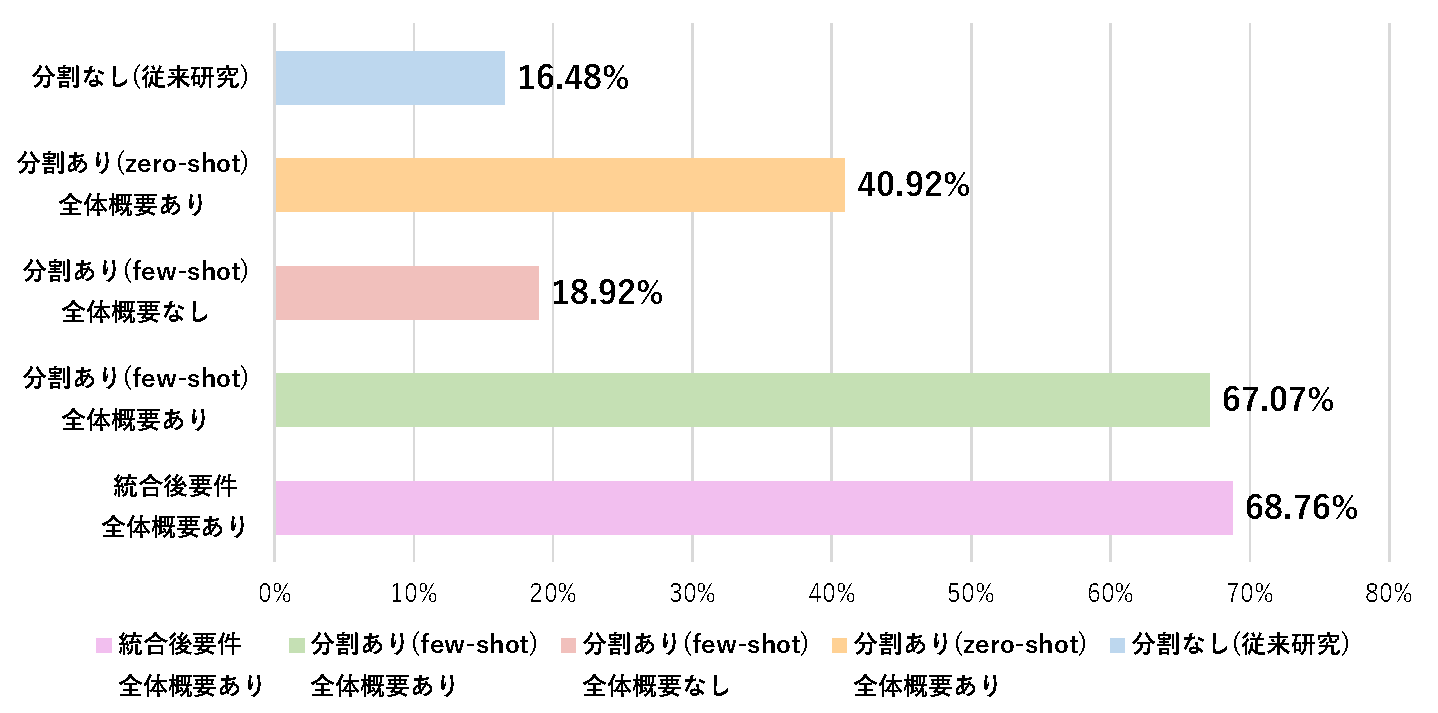
\includegraphics[width=1.0\linewidth]{./Toyoshima_fig/RQ1_and_RQ2.pdf}
    \caption{few-shot学習,全体概要の有無,統合によるテスト通過率比較}
    \label{ses2025}
\end{figure}
%-------------------

\subsection{RQ2: 細分化した要件の再統合は,生成するソースコードのテスト通過率に影響を及ぼすか?}

図\ref{ses2025}には,RQ1の結果に加え,RQ2の結果も示す.要件統合前のテスト通過率は67.07\%であるのに対し,統合後は68.76\%に向上した.また,図\ref{rq2_1}は,統合前後で成功または失敗したテストケース数をPassedまたはFailedの結果を示す.統合前のテストに成功し,統合後のテストも成功した場合「Passed\&Pass」とする.本RQにおいてテストを通過するとは,各問題で用意された入出力テストが全て通過したケースを指す.

統合前のテストに成功し,統合後のテストも失敗した「Passed\&Fail」となるケース,および統合前のテストに失敗し,統合後のテストで成功した「Failed\&Pass」となるケースは,全体の12.5\%であり,統合前後で変化のないケースに比べて少ないため,統合によるテスト通過率の優位的な差は確認出来なかった.

% 要件の統合により「劣化」したケース,FailedかつPassとなるケースは,「改善」されたケースであり,それ以外の2項目は統合が生成されるソースコードの品質に影響を及ぼさなかったケースと考えられる.
% それぞれの割合を確認すると,劣化・改善がみられたのは全体の12.5\%であり,概ね変化がみられないことが確認された.

% 以上のことから,テスト通過率は概ね横ばいであり,通過する問題の構成も大きく変化しないことから,提案する統合手法は,生成されるソースコードの品質を損なわせるものではない事が示唆される.

%-------------------
\begin{figure}[t]
    \centering
    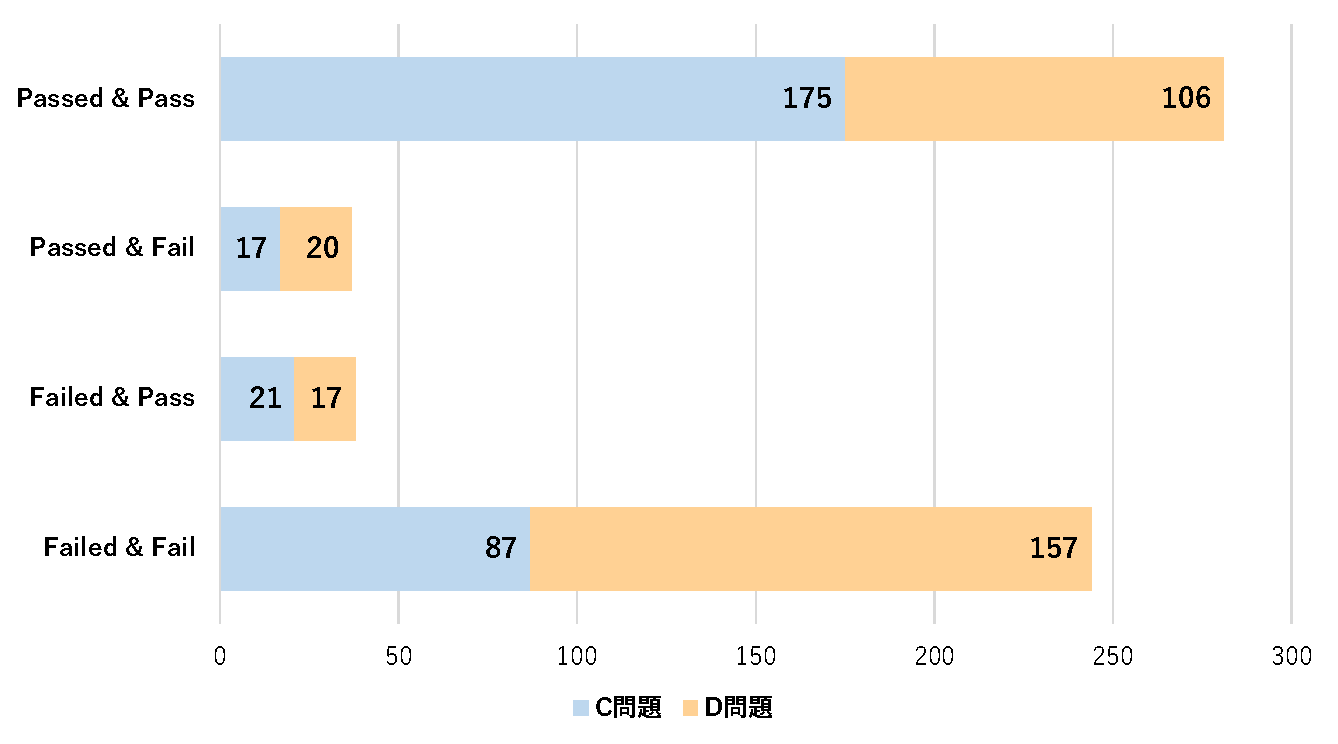
\includegraphics[width=1.0\linewidth]{./Toyoshima_fig/SIGSE_PF.pdf}
    \caption{統合前後のテスト通過問題数比較}
    \label{rq2_1}
\end{figure}
%-------------------

%\ihara{ここまで修正済み}

\subsection{RQ3: 再統合した要件からの要件の再分割は生成するソースコードのテスト通過率に影響を及ぼすか?}

RQ2において,要件を統合した場合においても,テストに通過した問題数に大きな変化は見られなかった.RQ3では,統合した要件をfew-shot学習の例として活用して,再分割した要件でソースコードを生成する実験を行った.few-shot学習では,統合前後の両方でテストを通過したケース(Passed\&Pass)のC問題とD問題よりそれぞれ4問ずつ,合計8問を使用し,再分割を実施する.
% 統合した品質の劣化が発生しないことが確認されたことから,統合前後の両方でテストを通過したケース(Passed かつ Pass)のケースより8件の分割例と問題文を抽出し,few-shot学習と再分割を実施した.
また,ソースコード生成にはfew-shot学習に使用する8問を除く,192問を対象に評価実験を行った.
% 分割例はC問題とD問題よりそれぞれ4問ずつ取得し,これらの問題は再分割・ソースコード生成のデータセットからは除外し,それぞれ96問ずつで実験を実施した.

RQ2で統合した結果をfew-shot学習し,要求を再分割することで,すべてのテストを通過した問題数の分布を図\ref{rq3_1}に,テスト通過率の比較した結果を図\ref{rq3_2}に示す.テストを全て通過した問題数は,C問題で延べ252問,D問題で延べ231問となり,RQ1において総テスト通過率67.07\%であったのが,再分割を行うことで87.59\%に向上した.また,改善が見られたケース(Failed\&Pass)が全体の36\%と通過したテストの半分近くを占める結果となった.

% RQ2で定義した問題単位のテスト結果の分布を図\ref{rq3_1}に示す.

% 用意されたテストを全て通過した問題数がC問題で252問,D問題で231問となり,総テスト通過率は83.85\%となることが確認された.又,改善が見られたケース(Failed かつ Pass)が全体の36\%と通過したテストの半分近くを占める結果となった.

% 以上より,本論文が提案する,統合に基づく要件の再分割は,要件に含まれる要求を正しく抽出できる可能性が示される.

\begin{figure}[t]
    \centering
    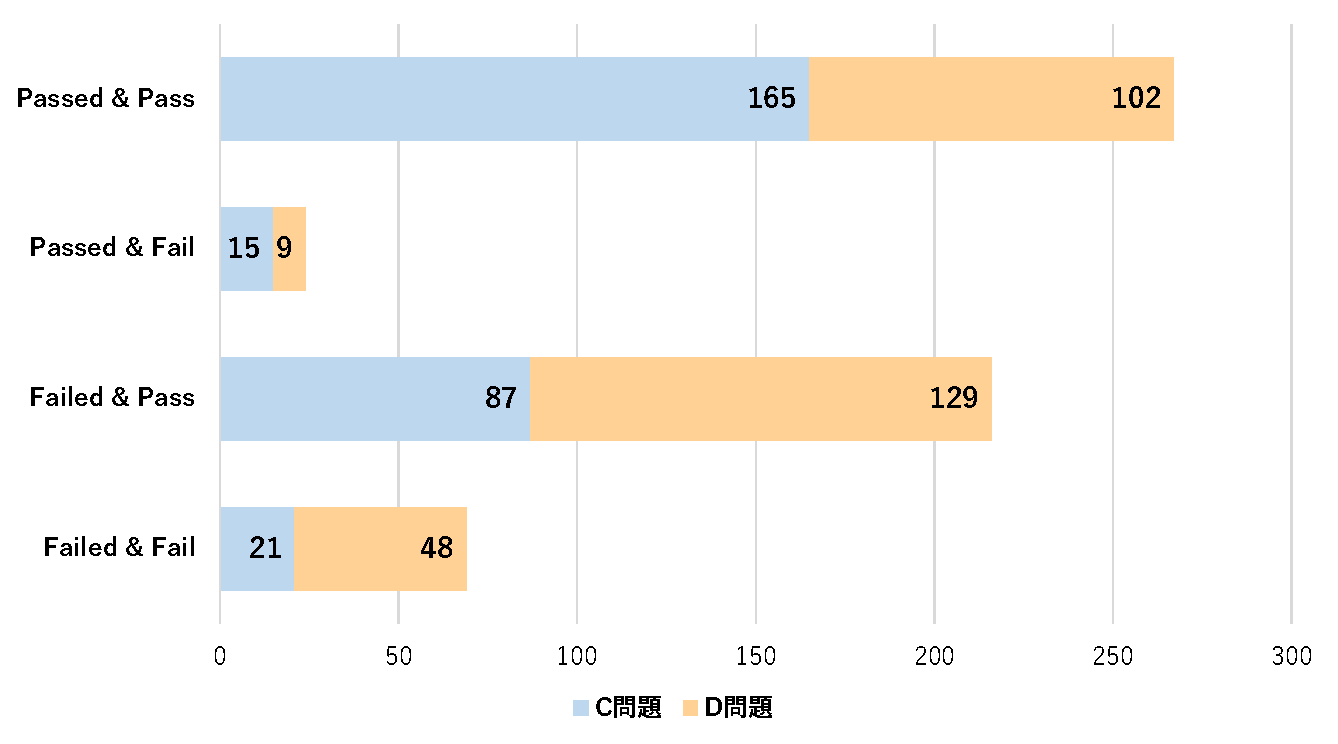
\includegraphics[width=1.0\linewidth]{./Toyoshima_fig/RQ3_1.pdf}
    \caption{再分割後のテストを通過する問題数比較}
    \label{rq3_1}
\end{figure}

\begin{figure}[t]
    \centering
    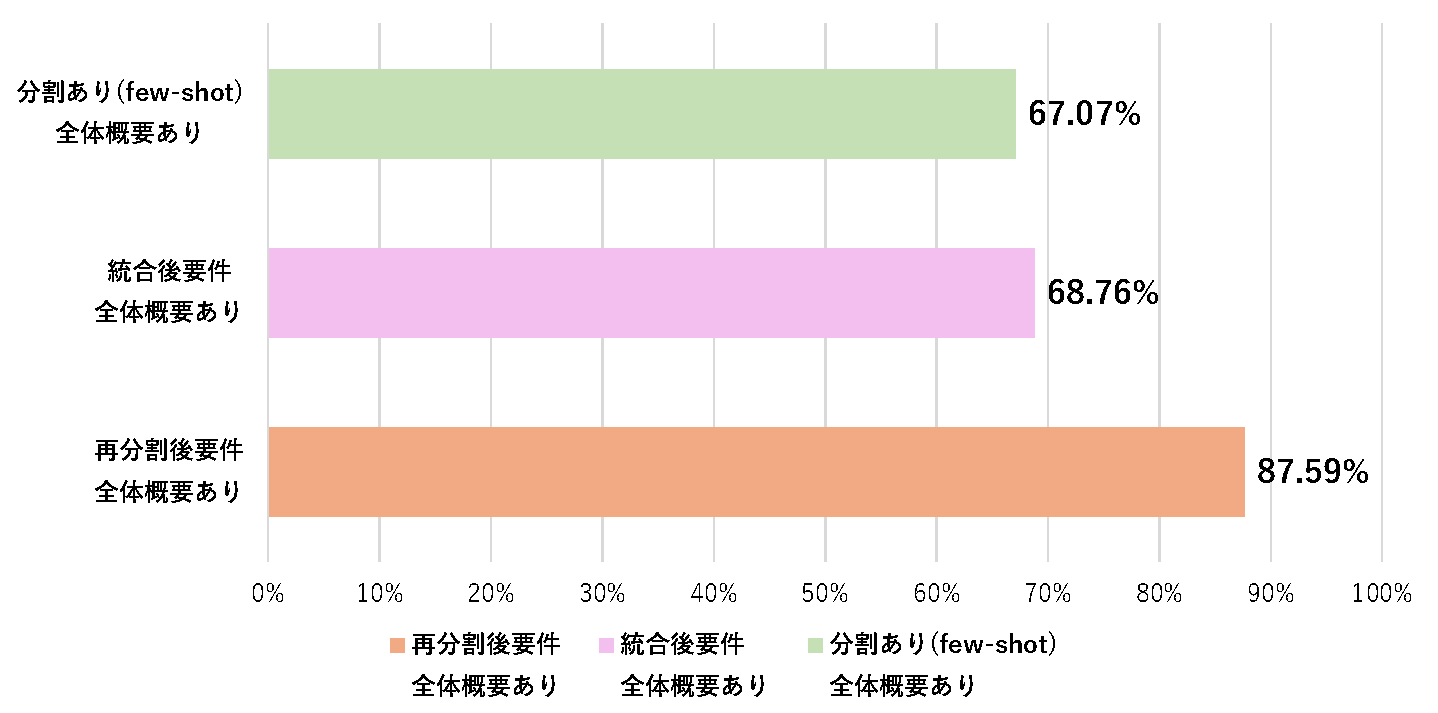
\includegraphics[width=1.0\linewidth]{./Toyoshima_fig/RQ3_2.pdf}
    \caption{統合前,統合後,再分割後で生成されるソースコードのテスト通過率比較}
    \label{rq3_2}
\end{figure}


%%%%%%%%%%%%%%%%%%%%%%%%%%%
%6
\section{考察}
\label{sec:discussion}
%%%%%%%%%%%%%%%%%%%%%%%%%%%
%6.1
\subsection{テスト通過率向上の要因分析}
本節では,AtCoderの問題に対するソースコード生成について,ChatDevを用いた要件分割,および統合によって,生成されるソースコードのテスト通過率が向上した理由を考察する.
6.1.1節では統合,再分割の前後のいずれにおいてもテストが通過した事例,6.2.2節では再分割を経てテストが通過するように変化した事例,をそれぞれ目視によって調査した結果を述べる.

%6.1.1
\subsubsection{統合前・統合後・再分割後の全てでテストを通過したケース}
本研究で扱った問題を対象に,統合前後・再分割後の全てにおいてテストを通過したケースの統合前後の要件文とそれにより生成されたソースコードを目視で比較した.

その結果,主な差異は要件の区切り方にみられた.
統合前では,変数・関数の宣言,値の代入,条件分岐の作成といった単発の作業のごとに要件が細かく分割でき,再分割後は宣言から初期化→関数の引き渡しなどのような意味的に連続した処理が1つの要件として束ねられ,それに対応するソースコードが生成できることを確認した.
したがって,機能は維持したまま,ソースコードを一度に生成しやすい最小単位のまとまりへ分割されたことが,テスト通過の要因である事が可能性として考えられる.

%6.1.2
\subsubsection{ケース2: 再分割により改善が見られたケース}
本ケースでは,要件の統合前,統合後でいずれも入出力テストに成功せず,再分割の実施後にテストを通過するようになった事例について目視で調査した.

統合によって,6.1.1節で述べた通り,要件1つあたりの区切られ方,即ち粒度が問題の構造に合わせて変化した.
加えて,再分割の過程では,これまで要件に反映しきれていなかった意図が要件レベルで明示されなかった事を確認した.具体的には,細かな値の更新や分岐制御,境界値の扱いや入出力形式,例外時の扱いなどが要件文内に含まれていた.

併せて,要件1つあたりの粒度が大きくなり,より少ない要件数で同等の内容を包含可能となった分,要求文より,各要件に含める細部の意図を具体化する事ができた.
したがって,工程間の繋ぎ目が減少し,前提や出力の解釈の揺らぎの抑制が行われ,意図が一貫して実装に反映されるようになった事が,入出力テストの通過に寄与した可能性が考えられる.



%6.2
\subsection{妥当性の脅威}
ChatDevと同様に,LLMエージェントによるソースコード自動生成が可能な別のフレームワークにおいても\cite{kiro},著者らが小規模な予備実験として複数問題において数回ずつのソースコード生成を実施したところ,要求文を満たさないソースコードが生成される事例が確認された.
このことから,要求文の仕様を満たさないソースコードの自動生成はChatDev特有の課題ではなく,LLMエージェントによるソースコード自動生成という領域全体に共通する課題であると考えられる.

LLMによるソースコード自動生成には再現性の欠如がある.同一のプロンプトを与えた場合においても,常に同一のソースコードが生成されるとは限らない.本研究では各問題に対してソースコード生成を3回行うことで再現性の高い結果が得られるよう努めた.
% 即ち,1度目の試行によって得られたソースコードが入出力テストを通過した場合でも,2度目の試行で生成されるソースコードが同一のテストを通過するとは限らない.このため,本研究で得られた結果は向上的に保証されるものではない点に留意する必要がある.
% \memo{ここまで田井くんが書いた内容をベースに作成しました.原文はコメントとして置いてあります.}
%\ChatDevと同じく、LLMエージェントによるソースコード自動生成が可能であるKiroにおいても、要求文を満たさないソースコードが生成される事例が確認された。これにより、要求文の仕様を満たさないソースコードの自動生成はChatDev特有の課題ではなく、LLMエージェントによるソースコード自動生成全体の課題であると考えられる。
%LLMによって自動生成されたソースコードの注意点として再現性の欠如が挙げられる。同一のプロンプトを与えた場合でも、常に同一のソースコードが生成されるとは限らない。つまり、1度の試行によって得られたソースコードが入出力テストを通過していたとしても、2度目の試行によって得られたソースコードが同じ入出力テストを通過するとは限らない。そのため、本研究によって得られた結果は保証できない点には注意が必要であると考えられる。
また,本研究はLLMとして,GPT-4o-miniのみで評価しており,学習データや推論モデルの異なる他モデルを使用した場合においても同様の検証が必要である.

本研究の評価対象は,主に競技プログラミングサイトであるAtCoderの問題群であり,非機能要件や状態管理,長期保守など多種多様な事象を留意すべき業務アプリケーションやソフトウェアなどの開発とは前提が異なる.
実装言語や環境なども限定的であり,それらが結果に与える影響については十分な検証が行われていない.
同様に,評価の中心指標として入出力サンプルの通過率を使用しているため,境界値の取りこぼしなどの可能性が拭いきれず,十分に要件を満たしたソースコードの生成が実施されているか否かは確認出来ていない.
また,few-shot学習において入力する例の選定や,
% 提示様式には研究者の裁量が入りやすく,
その内容や難易度,スタイルの差が通過率に影響を及ぼすことも示唆される.
加えて,データセットが公開されたものであるため,問題やその解法が既に学習済みである可能性と,それが結果に影響することも考えられる.

% 最後に,本研究で持ちた差分行数に基づく統合の閾値は,著者が経験的に定めたものであり,妥当性に関しては十分に検証されていない.閾値の選択が結果に与える影響について感度分析を含む追加の検証となる.

%%%%%%%%%%%%%%%%%%%%%%%%%%%
%7
\section{おわりに}
\label{sec:conclusion}
%%%%%%%%%%%%%%%%%%%%%%%%%%%
本研究では,LLMによるソースコード自動生成において,複数の要求を内包する複雑な要件に対して要件に対して生じがちな断片化と整合性の崩れの問題に着目し,few-shotによる要件の細分化と全体概要を与えた段階的実装,さらに生成結果に基づく要件の統合と再分割を実施する反復プロセスを提案した.

評価実験としては,RQ1で述べたようにfew-shotによる要件の細分化と,全体概要の共有を併用により,従来の一括生成や片方のみを導入した場合と比較して,した場合にテスト通過率が有意に向上した.
又,スナップショット差分行数に基づく要件の統合は品質の劣化を招かず,多くのケースで安定した挙動を示し,統合結果を新たな分割例として再分割を行う事によりテスト通過率の更なる向上が確認された.本手法は,全体整合性の担保と局所最適化に加え,自己最適化サイクルが有効に働く事を示唆する.

%ChatDevをベースとして開発を行う各ステップで分割された要件文と全体概要の学習により,それらを思考のガイドとしての役割を持たせながら開発の断片化を防ぐ事や,統合と再分割により,分割後の要件群の粒度最適化を図り,LLMフレンドリーな要件の粒度を模索する事が本研究の特徴と言える.
一方で,本研究の検証は競技プログラミングサイトの問題をベースに実施しており,様々な要素が複雑に絡み合う実務的開発へ流用可能であるかは追加検証が必要である.
また,LLMとして単一モデルを使用した事や,統合判定の閾値の根拠が乏しい事も課題として挙げられるため,今後はGitHubなどに公開されている小規模な実務的課題を持つリポジトリなどを対象として再現性の検証を実施すると共に,統合判定の閾値の最適化アプローチや,他モデルを用いることへの影響についても調査していく.


\bibliographystyle{ipsjunsrt}
\bibliography{bibsample}

\end{document}